\documentclass[11pt,a4paper]{article}

\usepackage[T1]{fontenc}
\usepackage[utf8]{inputenc}
\usepackage[english]{babel}
\usepackage[a4paper,top=2.3cm,bottom=2.35cm,left=2.5cm,right=2.5cm,headsep=12pt]{geometry}
\usepackage{amsmath,amssymb,mathtools}
\usepackage{enumitem}
\usepackage{eurosym}
\usepackage{graphicx}
\usepackage{xcolor}
\usepackage{microtype}
\usepackage{avant}
\usepackage{mathptmx}
\usepackage{titlesec}
\usepackage{fancyhdr}
\usepackage{mdframed}
\usepackage{tikz}
\usepackage{needspace}
\usepackage{hyperref}
\usetikzlibrary{arrows.meta,positioning}

\definecolor{PPEBurgundy}{RGB}{112,28,47}
\definecolor{PPENavarraRed}{RGB}{211,32,46}
\definecolor{PPEGold}{RGB}{185,143,57}
\definecolor{PPEAccentLight}{RGB}{248,235,238}
\definecolor{PPEInk}{RGB}{37,31,33}
\definecolor{PPEMuted}{RGB}{101,83,88}

\hypersetup{colorlinks=true,linkcolor=PPEBurgundy,urlcolor=PPEBurgundy}
\setlength{\parindent}{0pt}
\setlength{\parskip}{0.45em}
\setlist[itemize]{topsep=0.3em,itemsep=0.2em,leftmargin=1.5em}
\setlist[enumerate]{topsep=0.35em,itemsep=0.35em,leftmargin=1.9em}
\raggedbottom
\allowdisplaybreaks[2]

\titleformat{\section}
  {\sffamily\bfseries\large\color{PPEInk}}
  {\color{PPEBurgundy}\thesection}{0.8em}{}
\titlespacing*{\section}{0pt}{1.35em}{0.5em}

\newmdenv[
  skipabove=0.7em,skipbelow=0.85em,
  leftline=true,rightline=false,topline=false,bottomline=false,
  linewidth=3pt,linecolor=PPEBurgundy,backgroundcolor=PPEAccentLight,
  innerleftmargin=0.8em,innerrightmargin=0.8em,
  innertopmargin=0.55em,innerbottommargin=0.55em
]{solutionbox}

\newmdenv[
  skipabove=0.65em,skipbelow=0.75em,
  leftline=true,rightline=false,topline=false,bottomline=false,
  linewidth=2pt,linecolor=PPEGold,backgroundcolor=white,
  innerleftmargin=0.75em,innerrightmargin=0.75em,
  innertopmargin=0.45em,innerbottommargin=0.45em
]{tipbox}

\pagestyle{fancy}
\fancyhf{}
\fancyhead[LE,LO]{\sffamily\small Microeconomics \textbar{} Midterm Examination \textbar{} Worked solutions}
\fancyhead[RE,RO]{\sffamily\small\color{PPEBurgundy}\thepage}
\fancyfoot[C]{\sffamily\scriptsize\color{PPEMuted}Companion to the Midterm Examination, Chapters 1--10}
\renewcommand{\headrulewidth}{0.45pt}
\renewcommand{\headrule}{\hbox to\headwidth{\color{PPEGold}\leaders\hrule height \headrulewidth\hfill}}
\setlength{\headheight}{15pt}

\newcommand{\MRS}{\operatorname{MRS}}

\begin{document}

\begin{center}
  \IfFileExists{assets/branding/unav-logo-black.png}{%
    
\includegraphics[width=0.28\textwidth]{assets/branding/unav-logo-black.png}%
  }{%
    {\sffamily\bfseries\Large Universidad de Navarra}%
  }\par
  \vspace{0.5em}
  {\sffamily\color{PPENavarraRed}\large\textsc{Politics, Philosophy and Economics}\par}
  \vspace{0.3em}
  {\color{PPEGold}\rule{0.72\textwidth}{1.3pt}\par}
  \vspace{0.55em}
  {\sffamily\bfseries\color{PPEBurgundy}\LARGE Midterm Examination: Microeconomics\par}
  \vspace{0.16em}
  {\sffamily\large Worked solutions --- Chapters 1--10\par}
\end{center}

\begin{solutionbox}
\textbf{How to use this key.} The answers show the calculation and the
economic reasoning expected for full credit. Equivalent algebra, notation, and
clearly labelled diagrams should also receive credit.
\end{solutionbox}

\section{Derivatives \hfill (6 points)}

Let \(f(x)=2x^2+6x+40\) and \(g(x)=3x^4-4x^3+6x^2-8\).

\begin{align*}
\textbf{1.a}\quad f'(x)&=\boxed{4x+6}.\\[0.3em]
\textbf{1.b}\quad g'(x)&=\boxed{12x^3-12x^2+12x}.
\end{align*}

\textbf{1.c Product rule.} Since \(h(x)=f(x)g(x)\),
\[
\boxed{
h'(x)=(4x+6)(3x^4-4x^3+6x^2-8)
 +(2x^2+6x+40)(12x^3-12x^2+12x).
}
\]
There is no need to expand the two products.

\textbf{1.d Chain rule.}
\[
a'(x)=\frac12(2x^2+6x+40)^{-1/2}(4x+6)
=\boxed{\frac{2x+3}{\sqrt{2x^2+6x+40}}}.
\]

\textbf{1.e General power.}
\[
\boxed{b'(x)=\beta(2x^2+6x+40)^{\beta-1}(4x+6).}
\]

\textbf{1.f Quotient rule.} Let \(N=2x^2+6x\) and \(D=x^3-4x\). Then
\(N'=4x+6\) and \(D'=3x^2-4\), so
\[
\boxed{
i'(x)=\frac{(4x+6)(x^3-4x)-(2x^2+6x)(3x^2-4)}
{(x^3-4x)^2}.
}
\]

\section{Preference language and opportunity cost \hfill (14 points)}

\textbf{2.a} \(A\sim B\) means that the consumer is indifferent between
bundles \(A\) and \(B\): each is weakly preferred to the other.

\textbf{2.b} \(A\succ B\succeq C\) means that \(A\) is strictly preferred to
\(B\), and \(B\) is weakly preferred to \(C\). With transitive preferences,
it also follows that \(A\succ C\).

\textbf{3. Comparing the bundles.} The diagram gives
\[
A=(1,1),\qquad B=(5,1),\qquad C=(1,5),\qquad D=(5,5).
\]
Monotonicity implies
\[
\boxed{B\succ A,\qquad C\succ A,\qquad D\succ A.}
\]
The comparison between \(C\) and \(B\) cannot be determined from monotonicity
alone: each has more of one good and less of the other. Thus
\[
\boxed{\text{the relation between \(C\) and \(B\) is indeterminate.}}
\]

\textbf{4. Opportunity cost.} A textbook costs \(\text{\euro}12\), while a
notebook costs \(\text{\euro}3\). Therefore,
\[
\boxed{\text{one textbook costs 4 notebooks}}
\]
and
\[
\boxed{\text{one notebook costs }\frac14\text{ of a textbook}.}
\]

\section{Consumer choice I \hfill (10 points)}

\textbf{5.a Budget line.} The constraint is
\[
12x+4y=120
\qquad\Longleftrightarrow\qquad
\boxed{y=30-3x}.
\]
The intercepts are \((10,0)\) and \((0,30)\), and the slope is
\(-p_x/p_y=-3\).

\textbf{5.b Substitution into utility.} On the budget line,
\[
u(x)=x(30-3x)=\boxed{30x-3x^2}.
\]

\textbf{5.c Optimisation.}
\[
u'(x)=30-6x=0
\quad\Longrightarrow\quad
x^*=5.
\]
Then
\[
y^*=30-3(5)=15.
\]
Because \(u''(x)=-6<0\), this stationary point is a maximum. Hence
\[
\boxed{(x^*,y^*)=(5,15),\qquad u^*=75.}
\]

\begin{center}
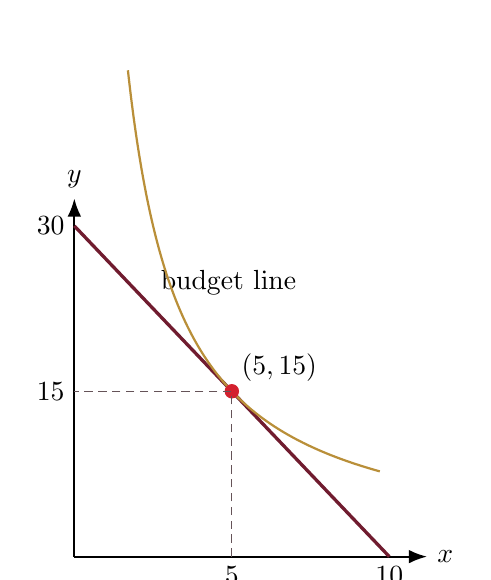
\begin{tikzpicture}[x=0.40cm,y=0.14cm,>=Latex]
  \draw[->,thick] (0,0) -- (11.2,0) node[right] {\(x\)};
  \draw[->,thick] (0,0) -- (0,32.5) node[above] {\(y\)};
  \draw[PPEBurgundy,very thick] (0,30) -- (10,0) node[pos=0.24,above right,black] {budget line};
  \draw[PPEGold,thick,domain=1.7:9.7,samples=90,smooth] plot (\x,{75/\x});
  \filldraw[PPENavarraRed] (5,15) circle (2.4pt) node[above right,black] {\((5,15)\)};
  \draw[densely dashed,PPEMuted] (5,0) -- (5,15) -- (0,15);
  \node[below] at (5,0) {\(5\)};
  \node[left] at (0,15) {\(15\)};
  \node[left] at (0,30) {\(30\)};
  \node[below] at (10,0) {\(10\)};
\end{tikzpicture}
\end{center}

\section{Consumer choice II \hfill (10 points)}

\textbf{6.a Budget line.}
\[
20x+10y=180
\qquad\Longleftrightarrow\qquad
\boxed{y=18-2x}.
\]
Its intercepts are \((9,0)\) and \((0,18)\), and its slope is \(-2\).

\textbf{6.b Marginal rate of substitution.}
\[
MU_x=\frac23x^{-1/3}y^{1/3},
\qquad
MU_y=\frac13x^{2/3}y^{-2/3}.
\]
Consequently,
\[
\MRS_{x,y}=\frac{MU_x}{MU_y}
=\boxed{\frac{2y}{x}}.
\]

\textbf{6.c Optimal choice.} At an interior optimum,
\[
\frac{2y}{x}=\frac{p_x}{p_y}=2
\quad\Longrightarrow\quad y=x.
\]
Substitution into the budget line gives
\[
20x+10x=180
\quad\Longrightarrow\quad
\boxed{x^*=6,\qquad y^*=6.}
\]

\section{Substitution and income effects \hfill (9 points)}

\begin{center}
\begin{tabular}{c|c|l}
Question & Answer & Reason \\ \hline
7 & \(\boxed{A}\) & \(A\) is the tangency on the original budget line \(RS\).\\
8 & \(\boxed{B}\) & \(B\) is the tangency on the new budget line \(RT\).\\
9 & \(\boxed{D}\) & \(D\) is the compensated optimum on the original indifference curve.\\
10 & \(\boxed{D\text{ to }B}\) & This is the income effect after the relative-price change.
\end{tabular}
\end{center}

\begin{tipbox}
\textbf{Interpretation.} The substitution effect changes the chosen bundle
because coffee has become relatively cheaper, holding utility at its original
level. The income effect then reflects the extra purchasing power created by
the lower coffee price.
\end{tipbox}

\section{Cost curves and competitive supply \hfill (8 points)}

For
\[
TC(q)=36+6q+q^2,
\]
\[
\boxed{FC=36},\qquad
\boxed{VC(q)=6q+q^2},\qquad
\boxed{MC(q)=6+2q}.
\]
Average fixed and variable costs are
\[
\boxed{AFC(q)=\frac{36}{q}},\qquad
\boxed{AVC(q)=6+q}.
\]

As a price-taking firm, the firm chooses output where \(p=MC\), provided that
it covers average variable cost:
\[
30=6+2q
\quad\Longrightarrow\quad
\boxed{q^*=12}.
\]
At \(q=12\),
\[
ATC(12)=\frac{36}{12}+6+12=\boxed{21},
\qquad
MC(12)=\boxed{30}.
\]

\section{Production and demand \hfill (15 points)}

\textbf{12. Returns to scale.}
\[
q(2L,2K)=2(2L)^{1/2}(2K)^{1/2}
=2\cdot2L^{1/2}K^{1/2}=2q(L,K).
\]
Doubling both inputs doubles output. The production function therefore has
\[
\boxed{\text{constant returns to scale}.}
\]

\textbf{13.a Price elasticity.} Rewrite demand as
\[
Q=24-\frac P2,
\qquad
\frac{dQ}{dP}=-\frac12.
\]
Thus
\[
\boxed{\varepsilon_{Q,P}=-\frac12\frac{P}{Q}
=-\frac{P}{2Q}.}
\]

\textbf{13.b Unit elasticity.} Set \(\varepsilon_{Q,P}=-1\):
\[
-\frac{P}{2Q}=-1
\quad\Longrightarrow\quad
P=2Q.
\]
Together with \(P=48-2Q\),
\[
2Q=48-2Q
\quad\Longrightarrow\quad
\boxed{Q=12,\qquad P=24.}
\]

\textbf{14.} Total revenue is maximised at unit elasticity:
\[
\boxed{\varepsilon_{Q,P}=-1.}
\]

\textbf{15. Revenue effect.} At \(P=\text{\euro}10\),
\[
Q=120-2(10)=100,
\qquad
\varepsilon_{Q,P}=-2\frac{10}{100}=\boxed{-0.2}.
\]
Demand is inelastic. A small price increase therefore
\[
\boxed{\text{increases total revenue}.}
\]

\textbf{16.} The cross-price elasticity of substitutes is
\[
\boxed{\text{positive}.}
\]

\section{Elasticity and rational preferences \hfill (8 points)}

\textbf{17.a Own-price elasticity of rice.}
\[
\varepsilon_{\mathrm{rice,rice}}
=\frac{+10\%}{-20\%}
=\boxed{-0.5}.
\]

\textbf{17.b Cross-price elasticity.}
\[
\varepsilon_{\mathrm{pasta,rice}}
=\frac{-5\%}{-20\%}
=\boxed{+0.25}.
\]

\textbf{17.c} Rice and pasta are
\[
\boxed{\text{substitutes, because the cross-price elasticity is positive}.}
\]

\textbf{18.} If price rises by 10\%, quantity demanded changes by
\[
(-0.5)(10\%)=\boxed{-5\%}.
\]
Quantity demanded falls by 5\%.

\textbf{19.} Three standard conditions are:
\begin{itemize}
  \item \textbf{Completeness:} any two bundles can be compared.
  \item \textbf{Transitivity:} if \(A\succeq B\) and \(B\succeq C\), then
        \(A\succeq C\).
  \item \textbf{Monotonicity:} more of an ordinary good, holding the other
        goods fixed, is preferred to less.
\end{itemize}
Other standard axioms such as reflexivity, continuity, or convexity should
also receive credit when accurately defined.

\section{Profit maximisation \hfill (5 points)}

\textbf{20.a Profit function.}
\[
\pi(q)=20q-(30+4q+q^2)
=\boxed{16q-30-q^2}.
\]

\textbf{20.b Optimal quantity.}
\[
\pi'(q)=16-2q=0
\quad\Longrightarrow\quad
\boxed{q^*=8}.
\]
Since \(\pi''(q)=-2<0\), this is a maximum.

\textbf{20.c Profit at the optimum.}
\[
\pi(8)=16(8)-30-8^2
=128-30-64
=\boxed{34}.
\]

\section{Key concepts \hfill (15 points)}

\begin{description}[style=nextline,font=\sffamily\bfseries,leftmargin=3.35cm]
  \item[Economics]
  The study of how people and societies allocate scarce resources among
  competing uses.

  \item[Opportunity cost]
  The value of the best alternative forgone when a choice is made.

  \item[Marginal analysis]
  Comparing the additional benefit and additional cost of a small change in a
  decision, such as one more unit of output.

  \item[Preference]
  An individual's ranking of possible bundles or outcomes.

  \item[Indifference curve]
  The set of bundles that give a consumer the same level of utility.

  \item[Marginal rate of substitution]
  The amount of one good a consumer is willing to give up for an additional
  unit of another good while holding utility constant.

  \item[Budget set]
  All bundles a consumer can afford, given income and prices.

  \item[Normal good]
  A good for which demand rises when income rises, holding prices fixed.

  \item[Price elasticity of demand]
  The percentage change in quantity demanded associated with a one-percent
  change in the good's own price.

  \item[Cross-price elasticity of demand]
  The percentage change in demand for one good associated with a one-percent
  change in the price of another good.

  \item[Production function]
  A relationship showing the maximum output obtainable from different
  combinations of inputs, given technology.

  \item[Marginal product]
  The additional output produced by one more unit of an input, holding other
  inputs fixed.

  \item[Fixed cost]
  A cost that does not vary with output in the relevant period.

  \item[Variable cost]
  A cost that varies with the quantity produced.

  \item[Marginal cost]
  The additional cost of producing one more unit of output.
\end{description}

\end{document}

